\documentclass[a4paper, 12pt]{report}


% package
\usepackage{kotex}
\usepackage{setspace}
\usepackage{graphicx}
\usepackage{hyperref}
\usepackage{geometry}
\usepackage{caption}
\usepackage{wrapfig}
\usepackage{longtable} % 테이블이 여러 페이지로 나눠지도록 지원하는 패키지 (선택 사항)
\usepackage[table,xcdraw]{xcolor}  % 색상 적용을 위한 패키지
\usepackage{titlesec}
\usepackage{tocloft}


% document setting
\renewcommand{\figurename}{그림}    % 그림 캡션을 한글로 변경
\renewcommand{\abstractname}{요약}  % 요약 제목을 한글로 변경
\renewcommand{\contentsname}{목차}  % 목차 제목을 한글로 변경
\renewcommand{\appendixname}{부록}  % 부록 제목을 한글로 변경
\setstretch{1.50}                  % 줄 간격 설정
\setlength{\parskip}{6pt}          % 문단 간격 설정
\setlength{\parindent}{0pt}        % 문단 들여쓰기 제거
\renewcommand{\arraystretch}{2.0} % 표 내 줄 간격을 1.5배로 설정
\captionsetup{font=small}          % 캡션 폰트를 'small'로 설정
\geometry{top=3cm, bottom=3cm, left=2.5cm, right=2.5cm}  % 여백 설정
\titleformat{\chapter}[hang]{\normalfont\huge\bfseries}{제 \thechapter\ 장}{1em}{}
\setlength{\cftbeforetoctitleskip}{0cm} % 목차 제목 위 여백

\title{국가공공 정보시스템 안전성 및 활용성 제고를 위한 차세대 암호체계 개발 보고서}
\author{김동현(Kim DongHyeon, wlswudpdlf31@kookmin.ac.kr)}
\date{\today}

\begin{document}


\maketitle

% \begin{abstract}
% \end{abstract}

\tableofcontents

%! subsection은 세미나를 위해 작성한 것으로, 없애거나 다른 제목으로 지울 예정.

%? 서론 스토리 진행이 자연스러운가?

\chapter{서론}

% - 많은 기업 내 직원들이 화상회의 서비스를 사용하고 있다. [1, 2]
% - 이들은 화상회의 영상 유출 사고로 피해를 받을 수 있다. [3, 4]
% - 화상회의용 워터마크로 피해를 줄일 수 있다. [5, 6]
% - 현재 화상회의용 워터마크에는 ~~한 것들이 있다. [7]
% - 이 워터마크들은 ~~한 한계가 있고, 이를 해결할 기술이 필요하다. [8, 9]

\section{배경}

\iffalse
    이 제품은 누구를 위한 것이고, 왜 그가 중요한가? - 기업을 위한 것. 많은 직원이 화상회의 서비스를 사용하고 있다.
    그는 어떤 문제가 있고, 이 문제가 왜 중요한가? - 화상회의 영상 유출 사고가 있다. 영상은 기업 자산이므로 피해를 받을 수 있다.
\fi
오늘날 많은 기업이 화상회의 서비스를 사용하고 있다. 기업은 코로나 엔데믹
이후에도 여전히 재택근무나 원격근무를 추진하고 있고, 화상회의 서비스를 사용하는
직원은 계속해서 증가하고 있다. 기업은 이런 상황 속에서 화상회의와 관련한 보안을
강화해야한다. 특히, 화상회의 영상 유출 사고는 기업에 큰 피해를 줄 수 있다. 

\iffalse
    이 제품은 무엇이며, 이 제품이 왜 중요한가? - 워터마크 기술이다. 워터마크 기술로 영상 유출을 예방하고 피해를 줄일 수 있다.
\fi
워터마크는 화상회의 영상 유출을 예방하고, 유출 피해를 줄일 수 있는
기술이다. 화상회의용 워터마크 기술은 일반적으로 화상회의 영상 소유권을 보호하기
위해 사용한다. 화상회의 화면에 회의를 개설한 사용자(이하 호스트) 정보를
워터마크로 삽입하면, 모든 회의 참석자가 워터마크가 포함된 화면만 볼 수 있다.
회의 참석자 중 누군가 화면을 녹화하고 영상을 유출하면, 유출 영상으로부터
워터마크를 추출하여 이 영상이 호스트의 것임을 보일 수 있다. 

\iffalse
    이 제품은 어떤 것이 있는가? - Zoom이 제공하는 워터마크 기술.
\fi
대표적인 화상회의 서비스 Zoom는 워터마크 기술을 사용자에게 제공하고 있다. Zoom
워터마크 기술은 호스트 이메일을 모든 회의 참석자 화면에 띄워 참석자가 이메일을 볼 수
있다. 그림 \ref{fig:zoom_wm}은 Zoom에서 워터마크 기능을 사용했을 때 보이는
화상회의 화면이다.
\begin{figure}[ht]
    \vspace{10pt}
    \centering
    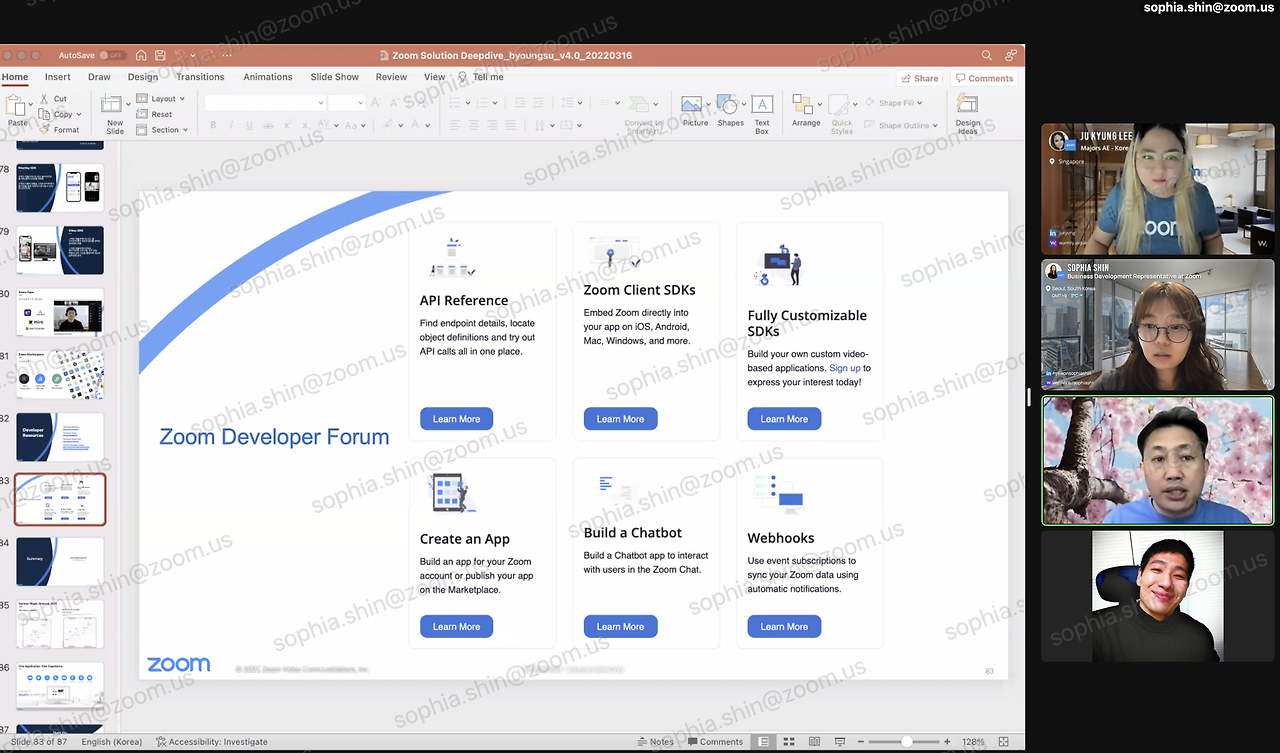
\includegraphics[width=0.7\textwidth]{imgs/zoom_wm.png}
    \caption{Zoom에서 워터마크를 삽입한 화상회의 화면}
    \label{fig:zoom_wm}
\end{figure}
Zoom 외에도 워터마크 기술을 제공하는 화상회의 서비스가 존재하며, 대부분 호스트의
식별정보를 워터마크로 사용한다. 이 워터마크 기술은 누군가 회의영상을
유출하더라도, 워터마크를 추출하여 영상 소유권이 호스트에 있음을 알 수 있다.
화상회의 서비스가 제공하는 워터마크 기술 외에도 많은 화상회의용 워터마크 기술이
존재한다. 이는 부록 \ref{apdx:aa}를 참고한다.

\section{목적}

\iffalse
    카멜레온 목적:
        1. 워터마크로부터 영상의 출처를 알 수 있도록 하기.
        2. 워터마크 메시지를 신뢰할 수 있도록 하기.
        3. 워터마크가 지워지지 않도록 하기.
    왜 이런 목적을 달성해야 하는지 설명해야한다. 기존 제품의 한계점을 언급할 수 있다.
\fi

기존 워터마크 기술에는 세 가지 한계점이 있다.

\begin{itemize}
    \item \textbf{출처 확인 불가능.} 기존 화상회의용 워터마크 기술은 회의 호스트
    식별 정보만 메시지로 사용한다. 호스트를 제외한 회의 참석자가 회의 화면을
    녹화하면, 녹화 영상에는 호스트 식별 정보만 워터마크로 삽입된다. 이 영상이
    유출되면, 유출 영상으로부터 호스트가 누구인지 알 수 있지만, 영상이
    어디로부터 유출됐는지, 누가 녹화한 영상인지 알 수 없다. 이 경우 유출 사고에
    대해 누구도 책임을 물을 수 없다. 또한 유출 출처를 막을 수 없어, 같은
    출처에서 또 다른 영상이 유출될 수 있다.
    \item \textbf{메시지 진위성 확인 불가능.} 워터마크는 신뢰할 수 있는 정보여야
    한다. 만약 워터마크에 들어가 있는 호스트 식별정보가 다른 사람의 식별정보로
    대체될 수 있다면, 유출 영상이 호스트의 것임을 확신할 수 없다. 기존
    워터마크는 메시지 진위성을 확인하는 과정이 없으므로, 워터마크를 신뢰할 수
    없다.
    \item \textbf{워터마크 삭제 가능.} 원본 영상을 손상하지 않고 워터마크를
    훼손하면, 워터마크 기능은 효력을 잃는다. 따라서 기존 워터마크는 쉽게 지울 수
    없도록 반투명화하여 콘텐츠에 삽입한다. 그러나 AI를 기반으로 한 워터마크 제거
    도구는 전문지식 없이도 기존 워터마크를 쉽게 지울 수 있다.[] 그림
    \ref{fig:wm_removed}는 AI 제거 도구를 사용하여 워터마크를 지운 화상회의
    사진이다.
    \begin{figure}[ht]
        \vspace{10pt}
        \centering
        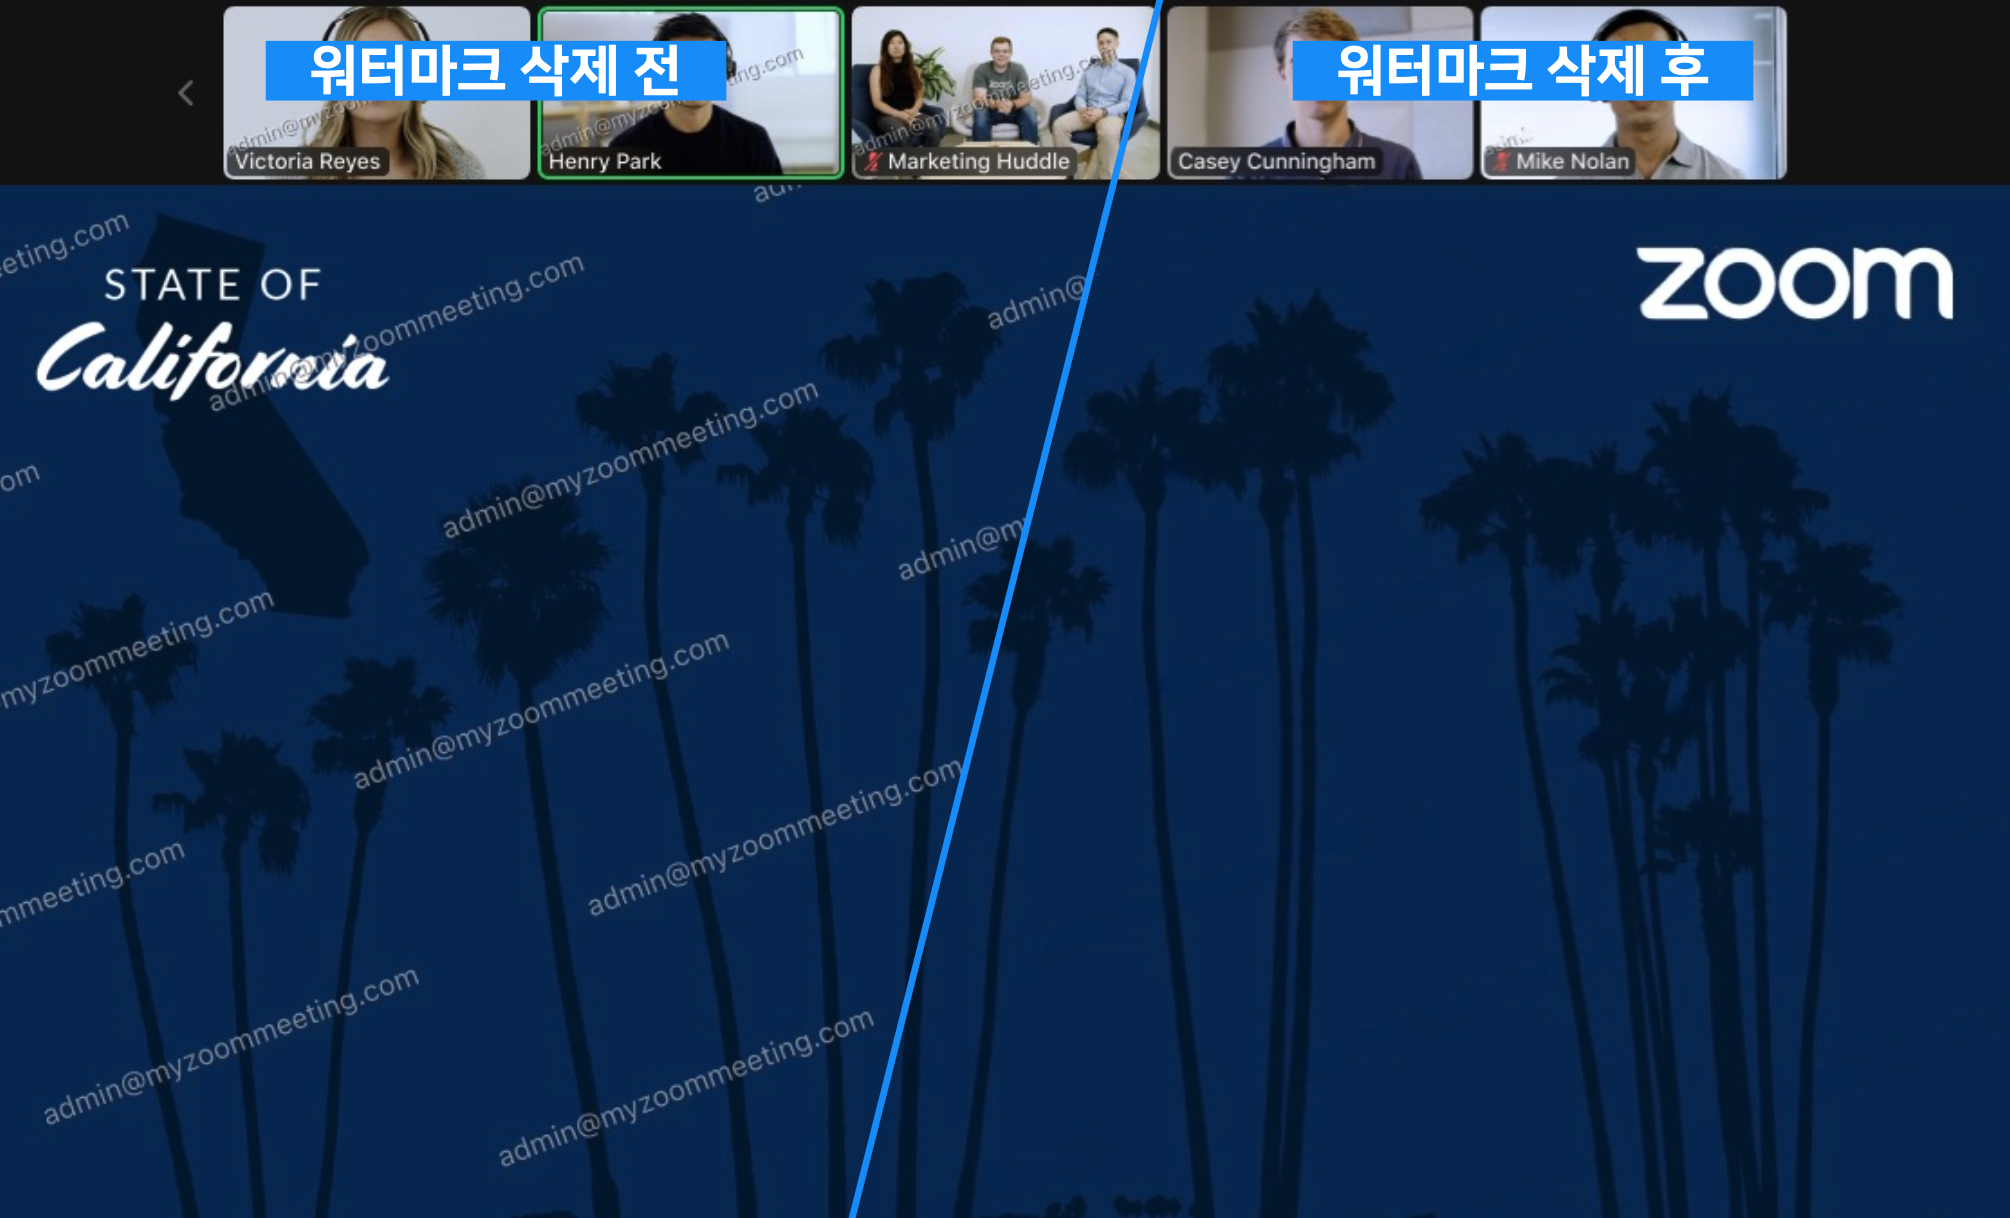
\includegraphics[width=0.7\textwidth]{imgs/wm_removed.png}
        \caption{AI 제거 도구로 Zoom 워터마크를 제거한 화상회의 화면}
        \label{fig:wm_removed}
    \end{figure}
\end{itemize}

화상회의 서비스 사용자가 기존 워터마크 기술을 사용하더라도 세 한계점 때문에
회의영상을 강하게 보호할 수 없다. 따라서 이를 해결하기 위한 개선된 워터마크
기술이 필요하다. 본 보고서에서 설명하는 워터마크 기술(이하 카멜레온)은 한계점을
극복한 개선된 워터마크 기술이다. 카멜레온은 출처와 진위성을 확인할 수 있고 AI
공격에도 견고하여, 기업은 화상회의 서비스를 보다 안전하게 사용할 수 있다.

\section{범위}

\iffalse
    카멜레온 범위:
        0. 이건 가능하다.
        1. 카멜레온은 카메라를 고려하지 않았다.
        2. 오디오 워터마크를 사용하지 않았다. 그러나 이는 독립적으로 개발 가능하다.
\fi
카멜레온은 호스트 정보뿐 아니라 회의 참석자 정보도 메시지로 사용한다. 유출한
회의영상이 가지는 워터마크로부터 참석자 정보를 확인하여 영상 출처를 알 수 있다.
카멜레온은 메시지의 진위성을 확인할 수 있는 정보를 생성하고, 워터마크로
삽입한다. 이 정보는 유출 영상에서 추출한 워터마크를 신뢰할 수 있는 증거라고 할
수 있다.

카멜레온은 AI 공격에 대응하기 위해 문자 형태 워터마크와 그림 형태 워터마크 두
가지를 사용한다. 문자 워터마크는 기존에 존재하는 워터마크 기술과 비슷하며, 그림
워터마크는 QR 코드를 활용한다. 두 종류 워터마크를 사용하면 AI는 두 워터마크를
전부 지우지 못하거나, 지우더라도 원본을 크게 훼손하여 영상 가치가 사라진다.
QR 코드 워터마크는 AI 공격 내성을 가질 수 있지만, PC 녹화기능이 아닌 외부에서
카메라로 녹화할 경우 추출이 어렵다.
\chapter{워터마크 형상}

카멜레온은 기존 화상회의용 워터마크 기술이 가지는 한계를 극복한 워터마크
기술이다. 카멜레온은 회의 호스트 정보 뿐만 아니라 회의 참석자 정보를 추가하여,
회의영상을 녹화하는 참석자가 누구인지 알 수 있다. 또한 워터마크 메시지에 MAC을
삽입하여 메시지의 진위성을 확인 할 수 있다. 카멜레온은 기존 워터마크 기술과
비슷한 방식으로 텍스트를 삽입했고, QR코드를 이용하여 그림 형태 워터마크를
삽입했다. QR코드 워터마크는 회의영상을 실시간으로 캡처하여 QR코드 색을 캡처한
사진의 색과 비슷하게 생성한다. 이를 통해 AI가 QR코드와 회의영상과 구분할 수 없게
했다.

\section{텍스트 워터마크}

텍스트 워터마크는 콘텐츠 이용자가 메시지를 그대로 볼 수 있는 워터마크이다.
텍스트 워터마크를 사용하여 회의 참석자가 회의를 녹화하고 유출하면 안된다는
경각심을 가질 수 있다. 따라서 기존 영상 화상회의 서비스가 제공하는 워터마크
기술과 비슷하게 텍스트 워터마크를 삽입했다. 그러나 기존 워터마크는 유출자를
식별하지 못하고, 진위성을 판별할 수 없다. 카멜레온은 기존 텍스트 워터마크
메시지에 유출자 정보와 MAC을 삽입하여, 이 문제를 해결했다. 그리고 AI 제거 도구가
텍스트 워터마크를 지우지 못하는 경우를 고려하여 텍스트의 형태를 설정했다.

\subsection*{메시지 구성}

% 어떤 메시지를 삽입했는가?
카멜레온은 워터마크 메시지로 주의 사항, 호스트 식별 정보, 참석자 식별 정보, 현재
시간, 메시지 인증 코드를 사용한다.

\begin{itemize}
    \item \textbf{주의사항.} 텍스트 워터마크는 회의 참석자에게 하고 싶은 말을
    전달할 수 있다. 참석자에게 화상회의를 녹화하지 말라는 주의사항을 전달하여,
    실수로 녹화하는 일이 없도록 한다. 카멜레온은 "Do Not Copy!"를 메시지로
    삽입했으며, 다른 메시지를 사용할 수 있다.
    \item \textbf{호스트 식별정보.} 화상회의 영상의 소유권은 호스트에게 있다.
    회의 영상이 유출됐을 때, 워터마크로부터 호스트 정보를 얻어 영상 소유권이
    호스트에게 있음을 증명할 수 있다. 
    \item \textbf{참석자 식별정보.} 회의 참석자 식별 정보는 각 참석자 PC마다
    서로 다르다. 회의영상이 유출되었을 때, 참석자 식별 정보를 확인하여 어느
    참석자의 PC에서 유출되었는지 확인할 수 있다.
    \item \textbf{현재시간.} 회의를 진행하고 있는 현재 시간을 워터마크 삽입하여,
    유출된 회의가 언제 진행한 회의인지 알 수 있다. 현재 시간은 실시간으로
    갱신하여 새로운 메시지를 삽입한다.
    \item \textbf{메시지 인증 코드.} 메시지 인증 코드(이하 MAC)는 데이터가
    변조되었는지 검증 할 수 있도록 데이터 뒤에 덧붙이는 코드이다. 코드를 생성할
    때는 호스트의 키를 사용하여, 호스트만 데이터 변조 여부를 알 수 있다.
    카멜레온은 호스트 식별 정보, 참석자 식별 정보, 현재 시간 세 개의 메시지에
    대해 MAC값을 계산한다. 회의영상이 유출되면, 호스트는 자신의 키를 사용하여
    워터마크 메시지의 MAC을 계산하고, 워터마크로 삽입된 MAC과 같은지 확인하여
    메시지 진위성을 확인한다.
\end{itemize}

그림 \ref{fig:text_wm}은 텍스트 워터마크를 삽입한 회의영상 사진 일부이다.
주의사항으로 ``Do Not Copy!"를 보여주어, 회의 참석자들에게 회의영상을 복사하지
말라고 권고한다. Alice는 회의 호스트, Bob은 회의 참석자 중 한명의 식별정보이다.
Bob이 아닌 다른 참석자의 회의 영상에서는 해당 부분이 다른 정보로 나타난다.
그리고 현재 시간 2024...가 나타나 있으며, 밑에는 Alice-Bob-현재시간에 대한 MAC
값을 삽입했다. 사용한 키는 호스트 Alice의 키이며, 여기서는 `chameleon'를 키로
사용하고, 알고리즘은 SHA256을 사용했다.
\begin{figure}[ht]
    \vspace{10pt}
    \centering
    
\includegraphics[width=0.6\textwidth]{imgs/text_wm.png}  % 이미지 파일명 (여기서는 예시 이미지 사용)
    \caption{텍스트 워터마크 구성}
    \label{fig:text_wm}
\end{figure} 


\subsection*{삽입 방식}

% 텍스트의 형태는 어떻게 되는가?
다양한 형태로 텍스트를 삽입해본 결과, 텍스트 워터마크가 회의영상 속 텍스트와
유사하면, AI 제거 도구는 텍스트 워터마크를 지우지 못한다. 혹은 지우더라도 원본을
크게 훼손한다. 따라서 폰트, 글자 크기, 글자 색 등을 결정할 때, 화상회의 화면에
주로 보이는 텍스트와 유사하게 구성했다. 일반적으로 화상회의에서는 문서를
보여주거나 발표자료를 보여주기 때문에, 이 때 자주 사용하는 글자 형태에 맞췄다.
그러나 이렇게 텍스트 워터마크를 삽입하면, 회의 참석자 또한 워터마크와 문서 속
텍스트와 구분하기 어려워 회의 참여가 불편할 수 있다. 따라서 텍스트 워터마크를
기울여 문서 내 글과 구분했다.

% 화면에 어떻게 삽입하는가?
텍스트 워터마크는 많이 삽입할수록 추출할 가능성이 높다. 화면을 가리지
않으려고 일부에만 워터마크를 삽입할 경우, 유출자는 해당 부분을 자르고 영상을
유출시킬 수 있다. 따라서 카멜레온은 텍스트 워터마크를 화면 전체에 골고루
삽입했다. 또한 카멜레온은 워터마크에 애니메이션 효과를 줬다. AI 워터마크 제거
도구는 화면의 특정 영역을 선택해 워터마크를 지우는 기능이 있다. 워터마크의
위치가 고정되면, 선택 영역이 좁아져 원본을 크게 훼손하지 않고 워터마크를 지울 수
있다. 워터마크 위치를 옮기면 선택 영역이 넓어진다. 또한 워터마크가 움직이기
때문에 화면을 계속 가리지 않는다. 


\section{QR 코드 워터마크}

QR코드는 2차원 매트릭스 바코드의 일종이다. QR 코드는 오류정정기법을 사용해,
코드를 일부 훼손하더라도 그 안에 있는 메시지를 유지할 수 있다. 워터마크는
콘텐츠가 시간이 지남에 따라 열화되면서 훼손될 수 있고, 유출자에 의해 훼손될 수도
있다. QR 코드를 이용하여 워터마크를 삽입하면, 이러한 훼손에도 워터마크 내
메시지를 추출할 수 있다. 카멜레온은 QR 코드의 특성을 활용하기 위해,
QR코드로 워터마크를 삽입한다.


\subsection*{메시지 구성}


QR코드 워터마크가 담는 메시지는 텍스트 워터마크와 동일하다. 주의사항을
제외한 참여자 식별정보, 유출자 식별정보, 현재시간, MAC값을 담는다. 다만, 4
가지 정보를 하나의 QR코드에 담지 않고, MAC값은 다른 QR코드로 만들어, 두 개의
QR코드를 만든다. QR코드 크기는 78px로, 44 바이트 메시지를 담을 수 있다.

그림 \ref{fig:qr_wm}는 카멜레온이  QR코드 워터마크를 삽입한 영상 일부이다. 왼쪽
위 QR코드와 오른쪽 QR 코드가 다른 것을 알 수 있는데, 각각 식별정보와 현재시간을
담은 QR코드, MAC값을 담은 QR코드이다.
\begin{figure}[ht]
    \vspace{10pt}
    \centering
    
\includegraphics[width=0.4\textwidth]{imgs/qr_wm.png}
    \caption{QR코드 워터마크 구성}
    \label{fig:qr_wm}
\end{figure} 

\subsection*{삽입 방식}

카멜레온은 QR코드를 삽입 하기 전 QR 코드 색상을 결정한다. 색상은 화상회의 화면에
의존한다. 화상회의 화면을 캡처한 후 QR 코드를 삽입할 위치에 해당하는 픽셀의 평균
RGB를 계산한다. 이 값을 QR코드 색으로 결정한다. 그림 \ref{fig:qr_wm_color}는
QR코드 워터마크 색상 변경 방식을 그림으로 표현한 것이다.
\begin{figure}[ht]
    \vspace{10pt}
    \centering
    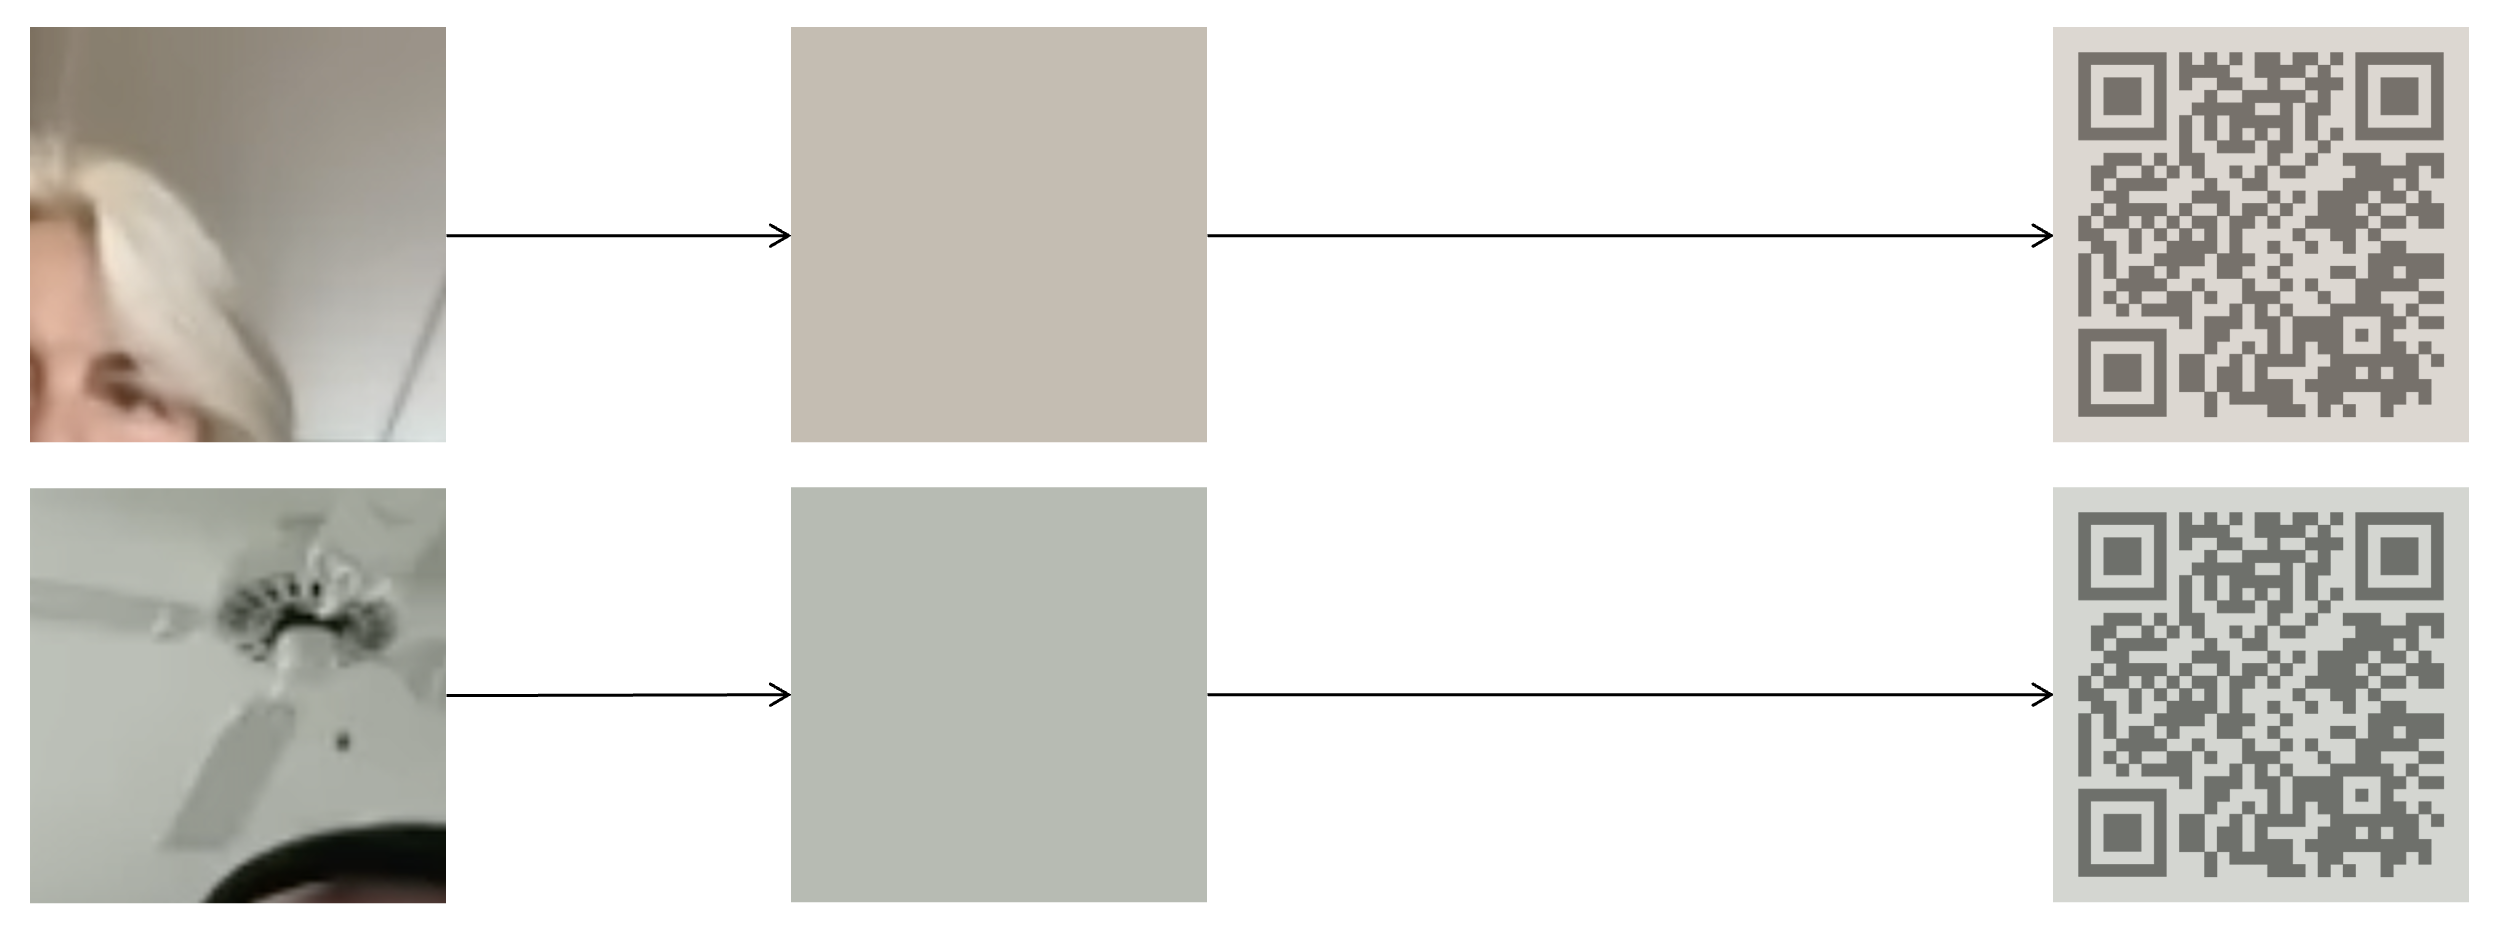
\includegraphics[width=0.8\textwidth]{imgs/qr_wm_color.png}
    \caption{QR코드 워터마크 색상 변경 방식}
    \label{fig:qr_wm_color}
\end{figure} 

이 방식은 두 가지 기대효과를 가진다. AI 워터마크 제거 도구는 QR코드 워터마크를
지울 수 있다. QR코드 색상을 화상회의 화면 색과 유사하게 변경하면 AI는 QR코드 워터마크와 화상회의
영상을 구분하지 못하기를 구분할 수 있다. 실험 결과, QR코드를 흑백으로 삽입했을
때보다, 색상을 비슷하게 만들어 삽입했을 때 AI는 덜 훼손하는 것을 확인했다.
그리고 QR코드를 화면 전체에 투사하면 회의 참석자는 QR코드에 의해 화면을 잘 보지 못할 수
있다. 따라서 QR코드 워터마크의 투명도를 높여 참석자가 회의영상을 시청할 때
불편함 을 줄일 수 있다. QR코드 색상을 뒷 배경 색과 비슷하게 만들면, QR코드의
투명도가 높아지는 효과를 줄 수 있다.

카멜레온은 두 종류의 QR코드를 화면에 체크무늬 형태로 출력한다. QR코드를 화면에 가득 채우면
회의에 방해가 될 수 있고, 향후에 비어있는 공간을 활용하여 다른 형태의
워터마크를 삽입할 수 있게 했다. 
\chapter{화상회의 적용}

이 절에서는 화상회의에서 카멜레온을 사용하여 워터마크를 삽입하고 유출
영상으로부터 워터마크를 추출하는 과정을 설명한다. 호스트가 서버에 회의 참석자
명단을 전달하면 서버는 워터마크 메시지를 생성하여 각 PC에 전달하고, 각 PC는
전달받은 메시지를 이용하여 워터마크 화면을 생성한다. 영상이 유출되면, 기업은
워터마크를 추출하여 호스트와 출처를 확인하고, 워터마크 메시지를 서버에 전달한다.
서버는 전달받은 메시지와 호스트 키를 사용하여 진위성을 확인할 수 있다. 이 절에서
설명하는 과정은 카멜레온을 사용할 수 있는 기본적인 방법 중 하나일 뿐, 반드시 이
과정을 준수할 필요는 없다.

\section{워터마크 삽입}

카멜레온이 워터마크 메시지를 생성하기 위해서는 카멜레온 서버는 모든 회의
참석자의 식별정보와 키를 가지고 있어야 한다. 이는 사전에 회원가입 등을 통해
얻는다. 호스트는 회의를 개설하고 카멜레온 서버에 회의 참석자 명단을 전달한다.
서버는 명단을 확인하고, 각 참석자 PC에 맞는 워터마크 메시지를 전달한다. 이 때
메시지는 사전에 가지고 있던 식별정보와 키를 이용하여 생성한다. 각 PC는 메시지를
텍스트 워터마크와 QR 코드 워터마크로 생성하여 화면에 출력한다. 이로써 모든 회의
참석자는 자신에 맞는 워터마크가 삽입된 회의 화면을 볼 수 있다. 그림
\ref{fig:wm_encoding}은 위 과정을 나타낸다.
\begin{figure}[ht]
    \vspace{10pt}
    \centering
    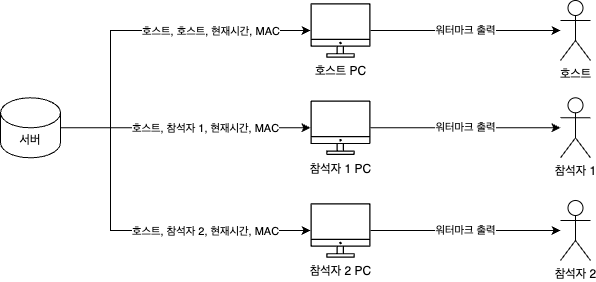
\includegraphics[width=0.7\textwidth]{imgs/wm_encoding.png}
    \caption{워터마크 삽입 과정}
    \label{fig:wm_encoding}
\end{figure}

\section{워터마크 추출}

유출영상이 심하게 훼손되었다면, 해당 영상은 가치가 없으므로 워터마크를 추출할
필요가 없다. 훼손이 적고, 텍스트 워터마크나 QR 코드 워터마크가 추출 가능할
정도로 남아 있다면, 이를 추출하여 소유자, 출처, 진위성을 확인할 수 있다.

해당 영상을 소유하고 있는 기업 또는 회의 호스트는 남아있는 워터마크를 추출 및
조합하여 워터마크 메시지를 생성한다. 메시지로부터 소유자와 출처를 확인할 수
있다. 진위성을 확인하기 위해 워터마크 메시지를 서버에 전달한다. 서버는 받은
메시지에서 호스트를 확인하고 이에 해당하는 키를 사용하여 MAC을 계산한다. 만약
계산한 값이 메시지 내 MAC과 일치한다면, 메시지 변조가 없음을 진위성 여부
요청자에게 알린다. 그림 \ref{fig:wm_decoding}는 위 과정을 그림으로 나타낸다.
\begin{figure}[ht]
    \vspace{10pt}
    \centering
    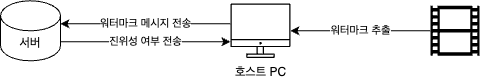
\includegraphics[width=0.7\textwidth]{imgs/wm_decoding.png}
    \caption{워터마크 추출 과정}
    \label{fig:wm_decoding}
\end{figure}
%! 성능 측정 방법에서는 지금 "대충 이런걸 적을 거에요"를 보여준 거고.
%! 성능 측정 결과에서는 지금 "성능 측정 결과, 이렇게 나왔습니다"를 보여준거다.
%! 이런 내용이 들어갈거에요 정도로 생각해야함.

\chapter{워터마크 성능}

(대충 여기가 뭐하는 장인지 적고, 이 장의 요약 적기)

\section{성능 측정 방법}

(넣은 이유: 성능 측정 결과에 신뢰성을 주기 위함.)

영상의 경우 성능을 측정하기 어려워, 영상 대신 이미지를 수집하여 워터마크를
삽입함. 워터마크가 삽입된 이미지로부터 워터마크가 얼만큼 추출되는지를 확인.

\begin{itemize}
    %? 더 필요한 내용이 있는가? 혹은 필요 없는 내용이나, 고쳐야 할 내용이 있는가?
    %? 구성방식의 문제?
    \item 이미지 수집
    \begin{itemize}
        \item \textbf{몇 개 수집했는가?} - 현재는 600개 (더 수집할 수 있음. 시간 오래 안걸림.)
        %? 1000개 딱 맞출까?
        \item \textbf{어떤 이미지를 수집했는가?} - PPT 사진, 문서 사진, 사람 얼굴이
        나오는 사진을 사용. 화상회의에서는 이러한 화면이 자주 나옴.
        %? 또 해봤으면 하는 사진이 있는가? 예를 들어, 자연 환경이라던가.
        %? 자연환경사진은 화상회의와 관련없지만 정확한 성능 측정에 도움이 될 수는 있다고 생각.
        %! 어떻게 수집했는가?에 대한 내용은 안넣었음.
        %! 사진 깃허브에 올리기: 굳이 안보여줘도 충분히 설득력 있는 글이 될 것이라 생각. 예시로
        %! 사진 몇 장 직접 만들어서 보여주는 것이 좋아보임.
    \end{itemize}
    \item 이미지 전처리
    \begin{itemize}
        \item \textbf{적절한 크기 이미지 사용.} 너무 작은(720p 미만) 이미지나 너무 큰(4k
        초과) 이미지는 제거.
        %! 여기를 <이미지 수집> 단계의 <어떤 이미지를 수집했는가> 단계에 넣을 수도 있음.
        %! 전처리할 내용이 적으면 그렇게 할 예정.
        %! 이미지를 AI를 활용해서 관련없는 이미지를 제거하거나 분류하는 건...시간 상 안될지도...
    \end{itemize}
    \item 워터마크 삽입
    \begin{itemize}
        \item \textbf{메시지와 키는 고정.}  성능 측정을 편하게 하기 위해 메시지와
        키를 -로 고정했음. 따라서 텍스트 워터마크와 qr코드 워터마크 형태는 변하지
        않으며, 모든 사진에 동일한 워터마크가 들어감.
        \item \textbf{애니메이션 효과 제거.} 텍스트 워터마크는 애니메이션 효과가
        있는데, 이는 제거함.
        \item \textbf{그 외에는 전부 동일.} 이전 장에서 설명한 방식과 동일하게
        워터마크 삽입. 투명도는 사용자 설정으로 조절 가능하니, 투명도를 어느정도
        주었는지 설명. 예시 보여주기.
        %! 깃허브에 워터마크 삽입 이미지 올릴수 있음.
        %? 추가 내용이 있을까?
        %! 어떻게 삽입했는가는 필요 없을 듯. 굳이 파이썬의 어떤 모듈을 이용해서 어쩌구 저쩌구. 그럴필요 있나?
        %! 프로토타입이니까 설명해야 할 것 같기도 하고.
    \end{itemize}
    \item 워터마크 훼손
    \begin{itemize}
        \item \textbf{노이즈 삽입.} AI 가 워터마크를 훼손했을 때 성능을 측정하기
        위함. 이미지 위에 작은 원을 골고루 뿌려 QR코드 워터마크를 훼손. 원
        크기를 키워서 크기에 따른 성능을 측정할 예정.
        \item \textbf{이미지 자르기.} 화상회의 화면은 겉을 조금 자르더라도
        가치있는(?) 화면이 될 수 있으므로, 공격자는 영상의 겉을 자를 수 있음.
        그리고 자른 만큼 워터마크가 사라지므로, 이에 대한 성능 측정이 필요.
        따라서 사진의 겉을 잘라서 성능을 측정. 점점 많이 잘랐음.
        \item \textbf{크기 조정.} (현재 이에 대해 성능 측정을 못해서 성능 측정이
        가능하면 적을 예정. 그러나 화상회의 영상은 시간이 지나면서 화질(?)이
        달라질 수 있으므로 이에 대한 워터마크 성능 측정을 하긴 해야함.)
    \end{itemize}
    \item 워터마크 추출 (현재 텍스트 워터마크 추출은 못한 상황...)
    \begin{itemize}
        \item \textbf{QR 워터마크를 어떻게 수집했는가?} QR코드 크기는 일정하기
        때문에 그리드 형태로 쉽게 자를 수 있음. 잘라서 QR코드가 위치한 부분만 모았음.
        \item \textbf{QR 코드 전처리} 자른 QR 코드 사진을 흑백으로 조정. 여기서
        바로 추출을 시도. 추출이 안된 QR코드는 Linear Filter를 이용하여 전처리
        후 다시 추출 시도. 예시 사진 보여주기. Linear Filter가 무엇인지 설명.
        \item \textbf{QR에서 메시지를 어떻게 뽑았는가?} 파이썬의 XX 모듈을 사용.
        (리더기 성능에 따라 추출이 될수도 있고 안될수도 있고 해서 이를
        넣어주었음.)
    \end{itemize}
\end{itemize}

\section{성능 측정 결과}

\iffalse
  어떤 내용을 넣을까? 추상적으로.
  - 추출이 잘 되는가?
    - 원본에서 추출이 잘 되는가?
    - 공격 후 추출이 잘 되는가?

  어떤 내용을 넣을까? 자세하게.
  - 

  영상이 손상되는 경우에는 뭐가 있을까?
\fi
\chapter{결론}

(위 장을 전부 작성한 후에 작성.)


\renewcommand{\bibname}{참고문헌}        % 제목을 한글로 변경
\addcontentsline{toc}{chapter}{참고문헌} % 목차에 포함
\begin{thebibliography}{99} % {99}는 항목의 번호 폭 설정

    \bibitem{latex-guide}
    (예시 1) L. Lamport, \textit{LaTeX: A Document Preparation System}, Addison-Wesley, 1994.
    
    \bibitem{knuth1984}
    (예시 2) D. E. Knuth, \textit{The TeXbook}, Addison-Wesley, 1984.
    
    % https://repository.kisti.re.kr/bitstream/10580/17881/3/ASTI%20MARKET%20INSIGHT%20027%280712%29.pdf

\end{thebibliography}

\appendix

\chapter{소스코드}
\chapter{동향}

(한국 등록특허 제10-2292595호 (2021.08.17) 작성 예정)


\end{document}